Nesse capítulo serão apresentados detalhes da implementação realizada nesse trabalho. O código foi desenvolvido em Python com auxílio da biblioteca PETSc (\citet{petsc-user-ref}). O PETSc é uma biblioteca famosa com diversas rotinas para computação científica, possui paralelismo utilizando MPI, estruturas de dados para matrizes esparsas, métodos de Krylov para solução de sistemas lineares, conjunto de pré-condicionadores (em particular os ILU), dentre outros. Estudos da performance da biblioteca podem ser encontrados em \citet{petsc-efficient}. O PETSc foi utilizado com a linguagem Python através dos \textit{bindings} disponibilizados no petsc4py (\citet{Dalcin2011}). O código aqui apresentado foi desenvolvido em sequencial. 


\section{Estrutura de Classes}

Primeiramente, foi necessário desenvolver uma estrutura para resolver problemas através do método dos elementos finitos, para depois realizar a implementação com o método multiescala. Esse desenvolvimento possui três principais classes: \textbf{Element}, \textbf{Node}, \textbf{FemContext}. As responsabilidades das classes são descritas abaixo:

\begin{itemize}
    \item \textbf{Node}: essa classe tem como intuito representar os nós do problema de elementos finitos. Guarda como propriedade as coordenadas x, y correspondentes, uma numeração global associada ao grid fino e se o nó pertence ou não a uma fronteira com condição de Dirichlet.
    \item \textbf{Element}: essa classe tem como intuito representar os elementos do problema de elementos finitos. Tem referência para os nós que pertencem ao elemento, guarda os valores do coeficiente de Young e Poisson, sabe calcular as funções de forma em coordenadas locais conforme \eqref{eq:definicaofuncform} e também é responsável por calcular a matriz do elemento local conforme \eqref{eq:matrizelemento}.
    \item \textbf{FemContext}: essa classe tem como intuito representar um problema de elementos finitos. Ela possui o conjunto de elementos e nós do problema em questão. Dá a numeração de cada um dos graus de liberdade dos nós. Calcula a matriz de rigidez através do Algoritmo \ref{alg:buildmatrix} e o lado direito correspondente. 
\end{itemize}

Essas três classes conjuntamente são capazes de montar e solucionar um problema de elementos finitos. Um fato importante é que a classe \textbf{FemContext} é responsável pela numeração dos graus de liberdades, pois, para calcular as funções de base, diferentes problemas locais tem que ser resolvidos e diferentes numeração locais são necessárias. Em uma implementação mais clássica de elementos finitos, o mais natural seria a numeração do grau de liberdade estar associada com a classe \textbf{Node}.


\section{Montagem dos Operador Multiescala}

Para a implementação do método multiescala, foi criada a classe \textbf{Multiscale}, essa classe tem como responsabilidade receber um objeto \textbf{FemContext} que representa o grid fino e calcular os operadores de prolongamento ($\mathbf{P}$), restrição ($\mathbf{P}^T$) e operador grosso ($\rigidmatrixcoarse$).


O primeiro passo para utilizar o método multiescala é a escolha do nível de engrossamento. A implementação aceita diferentes fatores para a direção x e y, apesar dos testes serem apresentados com o mesmo fator. O método \textbf{CoarseContext} da classe \textbf{Multiscale} é responsável por realizar a tarefa de construir $\mathbf{P}$ e $\rigidmatrixcoarse$. Essa tarefa é dividida nos seguintes passos: 

\begin{itemize}
    \item Criar objetos \textbf{FemContext} para cada um dos elementos grossos $\coarseelement$.
    \item Adicionar os nós e elementos correspondentes em cada um dos seus respectivos \textbf{FemContext}
    \item Para cada \textbf{FemContext} calcular a matriz de rigidez $\rigidmatrixelementms$.
    \item Resolver os oito problemas associados as funções de base encontrando $\basefunctionelemcoarse[1],  \basefunctionelemcoarse[2], \hdots, \basefunctionelemcoarse[8]$.
    \item Fazer o Assembly do operador de prolongamento.
    \item Calcular $\rigidmatrixcoarse = \mathbf{P}^T \rigidmatrix \mathbf{P}$
\end{itemize}

A Figura \ref{fig:esquemaconstrucao} apresenta um esboço da construção desse operador. Pode-se perceber que os problemas de cada \textbf{FemContext} são independentes, exceto pela solução dos problemas das arestas em comum. A implementação desse trabalho resolveu as arestas da fronteira duas vezes, uma implementação mais otimizada pode resolver apenas uma vez cada problema de fronteira. Em relação a resolver os oito problemas locais, foi realizada a fatoração LU da matriz que foi reaproveitada para a solução desses problemas. 

\begin{figure}[!htbp]
\centering
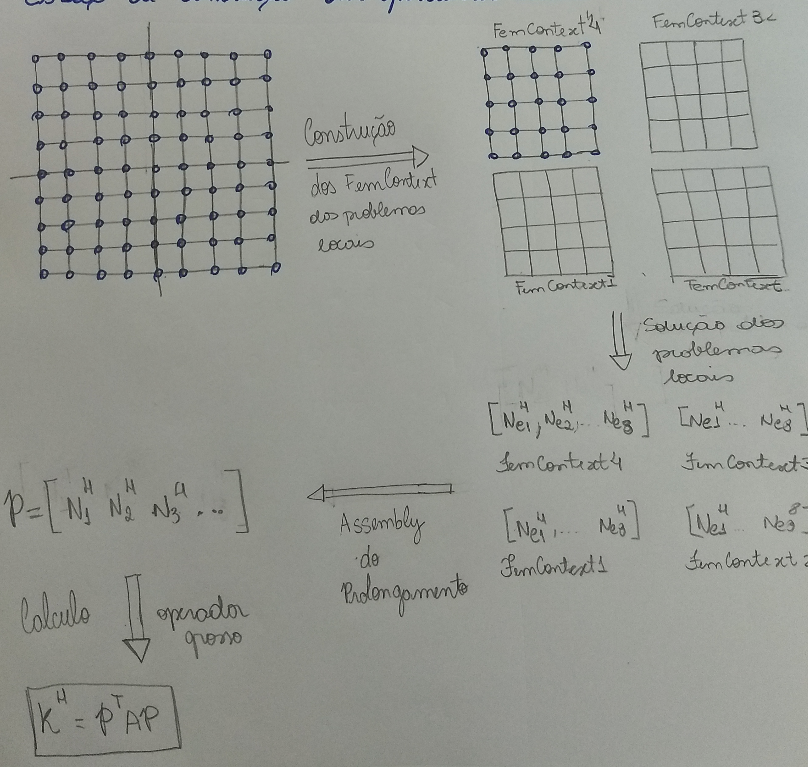
\includegraphics[width=\textwidth]{chap07/figs/esquemaprolongamento.png}
\caption{Esquema de construção dos operadores grossos. Mostrando um grid 8x8 sendo descomposto em um grid grosseiro 2x2 onde cada elemento grosso é formado por 4x4 elementos finos.}
\label{fig:esquemaconstrucao}
\end{figure}


O cálculo das matrizes dos operadores locais $\rigidmatrixelementms$ tem os mesmos coeficientes presentes na matriz de rigidez $\rigidmatrix$ visto que o operador de \eqref{eq:edp_geomec} é o mesmo de \eqref{eq:operadorlocal}. Assim, para o código executar mais rápido a matriz de rigidez de cada elemento foi armazenada para não precisar ser calculada novamente, isso torna o custo da memória maior, pois esses valores não precisam ser necessariamente guardados. Outra opção é perceber que a matriz de um operador local é uma submatriz do operador original e, portanto, poderia ser utilizado o método \textbf{GetSubMatrix} das matrizes do Petsc para construir $\rigidmatrixelementms$ a partir de $\rigidmatrix$ conforme mostra a Figura \ref{fig:submatrix}. Essa ideia é similar a utilizar uma reordenação Wire-Basket como apresentada em \cite{casteletto} e \cite{irina}.

\begin{figure}[!htbp]
\centering
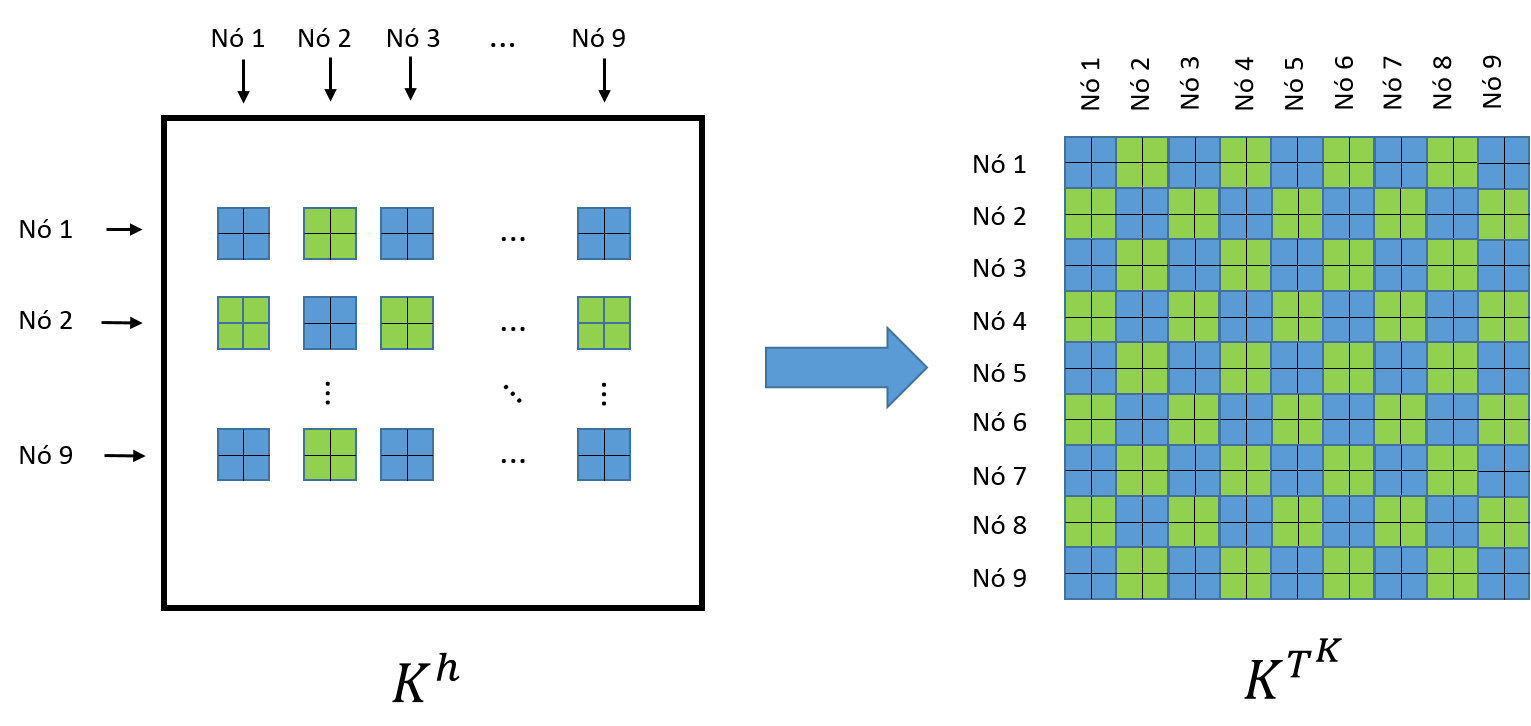
\includegraphics[width=\textwidth]{chap07/figs/submatrix.png}
\caption{Exemplo de construção de uma matriz relacionada a um problema local através do \textbf{GetSubMatrix}.}
\label{fig:submatrix}
\end{figure}


A classe \textbf{Multiscale} também possui um método solve, que só pode ser chamado após o método \textbf{CoarseContext} ter sido executado. Esse método recebe como entrada um vetor $\mathbf{f}^h$ relacionado a um lado direito do grid fino e resolve o problema no grid grosso e retorna para o grid fino. Em outras palavras, esse método retorna o seguinte valor $\mathbf{P}(\rigidmatrixcoarse)^{-1}\mathbf{P}^T \mathbf{f}^h$. Para a solução do sistema $(\rigidmatrixcoarse)^{-1}$ a solução utilizada foi uma fatoração LU. Essa fatoração é guardada para ser utilizada entre as iterações do método de Krylov quando o objeto o método \textbf{Multiescala} está sendo utilizado como pré-condicionador.

                                                                                   